%===========================================================================================================
\section{Motivation}
%===========================================================================================================
\begin{frame}{Why studying electroweak penguins and radiative $\boldsymbol{B}$ decays?}
\bi
\item {\footnotesize Flavor-changing neutral-current transitions $b\to s$ forbidden at tree level in the standard model.}
\itemii {\footnotesize Resulting $B$ decays are rare (loop or box diagrams):}
\bi
\itemiii {\footnotesize Branching fractions $\mathcal{B}\approx\mathcal{O}(10^{-7})\sim\mathcal{O}(10^{-4})$.}
\ei
\itemii {\footnotesize New physics may affect measured branching fractions and angular distributions of final-state particles.}
\ei
\vspace{0.1cm}
\centering
\includegraphics[width=0.32\linewidth]{figs/feynman/feynman_loop_charged.pdf}
\includegraphics[width=0.32\linewidth]{figs/feynman/feynman_loop.pdf}
\includegraphics[width=0.32\linewidth]{figs/feynman/feynman_loop_radiative.pdf}
\end{frame}
%===========================================================================================================
\section{The Belle II experiment}
%===========================================================================================================
{
  \usebackgroundtemplate{%
    \begin{picture}(100,100)(-190,70)
      \includegraphics[width=0.5\linewidth]{figs/superkekb}
    \end{picture}
  }
\begin{frame}{The SuperKEKB $\boldsymbol{B}$ factory}
\bi 
\item {\small \epem collider in Tsukuba, Japan.}
\itemii {\small $\sqrt{s}=10.6\gev=\mathrm{m}(\Y4S)$.}
\itemii {\small $\mathcal{B}(\Y4S\to\BB)>96\%$.}
\itemii {\small $\displaystyle\int_{25.03.2019}^{22.06.2022}\,\mathcal{L}_{\sqrt{s}=\mathrm{m}(\Y4S)}\,\mathrm{dt}=362\invfb$.}
\bi
\itemii {\small $N_{\BB}=3.87\times10^8$.}
\itemii {\small Similar to Babar sample and half of Belle’s.}
\ei
\itemii {\small Maximum instantaneous luminosity: $4.7\times10^{34}\cms$ (world record).}
\itemii {\small Target instantaneous luminosity: $6\times10^{35}\cms$.}
\ei
\end{frame}
}
%===========================================================================================================
\begin{frame}{{Strengths of Belle II for EW penguins and radiative $\boldsymbol{B}$ decays}}
\bi
\item {\footnotesize Belle II suited for measurements with neutral or missing energy.}
\bi
\itemiii {\footnotesize Knowledge of initial energy-momentum in \epem collisions.}
\itemiii {\footnotesize Moderate backgrounds.}
\itemiii {\footnotesize Close to $4\pi$ coverage.}
\itemiii {\footnotesize Photons: high detection efficiency and good energy resolution.}
\ei
\item {\footnotesize Good and similar identification of electrons and muons. \hfill \href{https://docs.belle2.org/record/2895/files/Lepton_identification_Moriond_2022__v2.pdf}{\tiny [BELLE2-CONF-PH-2022-003]}}
\ei
\vspace{0.25cm}
\begin{columns}
\begin{column}{0.5\linewidth}
\centering
\includegraphics[width=0.9\linewidth]{figs/belleii_new.pdf}
\end{column}
\begin{column}{0.5\linewidth}
{\tiny Photon-detection efficiency \href{https://docs.belle2.org/record/2604/files/BELLE2-NOTE-PL-2021-008.pdf}{\tiny [BELLE2-NOTE-PL-2021-008]}}
\centering
\includegraphics[width=0.85\linewidth]{figs/photon_efficiency.pdf}
\end{column}
\end{columns}
\end{frame}
%===========================================================================================================
\section{Electroweak penguins and radiative $\boldsymbol{B}$ decays}
%===========================================================================================================
\begin{frame}{Identifying $\boldsymbol{\BB}$-meson production}
\bi
\item {\footnotesize Knowing that $B$ mesons are produced in $\epem\to\Y4S\to\BB$ events is valuable.}
\item {\footnotesize When missing kinematic information in the signal decay ($B\to K \nunub$, inclusive $\B\to X_s\g$), accompanying $B$ ($B_{\mathrm{tag}}$) is used to constrain the signal.}
\ei
\vspace{0.1cm}
\centering
\includegraphics[width=0.6\linewidth]{figs/bsig_btag.pdf}
\bi
\itemiii {\footnotesize Hadronic tagging: $B_{\mathrm{tag}}$ is reconstructed in a hadronic decay. \hfill \href{https://doi.org/10.1007/s41781-019-0021-8}{\tiny [Comp Soft Big Sci 3, 6 (2019)]}}
\bi
\itemiii {\footnotesize Small tagging efficiency $\approx 0.1\%\sim0.5\%$, full kinematic information.}
\ei
\itemiii {\footnotesize Inclusive tagging: no explicit reconstruction of $B_{\mathrm{tag}}$. \hfill \href{https://doi.org/10.1103/PhysRevLett.127.181802}{\tiny [PRL 127 (2021) 18, 181802]}}
\bi
\itemiii {\footnotesize High tagging efficiency, limited kinematic information.}
\ei
\ei
\end{frame}
%===========================================================================================================
\begin{frame}{EW penguins and radiative $\boldsymbol{B}$ decay studies at Belle II}
\bi
\item {\footnotesize A variety of $b\to s$ processes test the standard model in different ways.}
\bi
\itemiii {\footnotesize In this talk.}
\itemiii {\footnotesize \color{lightgray} Not in this talk.}
\ei
\itemiii {\footnotesize Larger branching fraction of $\B\to X_s\g$ allows to study it with limited dataset.}
\ei
\centering
\vspace{0.25cm}
\resizebox{1.0\linewidth}{!}{
\begin{tabular}{llllll}
\toprule
& Decay & $\mathcal{O}(\mathcal{B})$ & Note & Dataset [$\invfb$] & Documentation \\
\midrule
\includegraphics[width=0.1\linewidth]{figs/feynman/feynman_loop_radiative.pdf} & Fully inclusive $\B\to X_s\g$ & $10^{-4}$ & hadronic tagging & 189 & \scriptsize \href{https://arxiv.org/abs/2210.10220}{[2210.10220]} \\
\includegraphics[width=0.1\linewidth]{figs/feynman/feynman_jpsi.pdf} & $B \to J/\psi(\ellell) K$ & $10^{-4}$ & control, \textit{not $b \to s$} & 189 & \scriptsize \href{https://arxiv.org/abs/2207.11275}{[2207.11275]} \\
\includegraphics[width=0.1\linewidth]{figs/feynman/feynman_loop_charged.pdf} & $\B\to\Kstar(892)\ellell$ & $10^{-6}$ & - & 189 & \scriptsize \href{https://arxiv.org/abs/2206.05946}{[2206.05946]} \\
& \color{lightgray} $\Bp\to\Kp\nunub$ & \color{lightgray} $10^{-6}$ & \color{lightgray} inclusive tagging & \color{lightgray} 63 & \color{lightgray} \scriptsize \href{https://doi.org/10.1103/PhysRevLett.127.181802}{[PRL 127 (2021) 18, 181802]} \\ % untagged
& \color{lightgray} $\B\to\Kstar(892)\g$ & \color{lightgray} $10^{-6}$ & \color{lightgray} - & \color{lightgray} 63 & \color{lightgray} \scriptsize \href{https://arxiv.org/abs/2110.08219}{[2110.08219]} \\
& \color{lightgray} $\Bp\to\Kp\ellell$ & \color{lightgray} $10^{-7}$ & \color{lightgray} - & \color{lightgray} 63 & \color{lightgray} \scriptsize \href{https://docs.belle2.org/record/2310/files/BELLE2-NOTE-PL-2021-005.pdf}{[BELLE2-NOTE-PL-2021-005]} \\
& \color{lightgray} Fully inclusive $\B\to X_s\g$ & \color{lightgray} $10^{-4}$ & \color{lightgray} - & \color{lightgray} 63 & \color{lightgray} \scriptsize \href{https://docs.belle2.org/record/2302/files/BELLE2-NOTE-PL-2021-004.pdf}{[BELLE2-NOTE-PL-2021-004]} \\ % untagged, https://docs.belle2.org/record/2208?ln=en
\bottomrule
\end{tabular}
}
\end{frame}
%===========================================================================================================
\section{Fully inclusive $\boldsymbol{\B\to X_s\g}$ \\ \hfill \includegraphics[width=0.5\linewidth]{figs/feynman/feynman_loop_radiative.pdf}}
%===========================================================================================================
\begin{frame}{Fully inclusive $\boldsymbol{\B\to X_s\g}$ with hadronic tagging I \hfill \href{https://arxiv.org/abs/2210.10220}{[2210.10220]}}
\bi
\item {\footnotesize Sensitive to new physics (differently from $b\to s\ell\ell$).}
\item {\footnotesize Unique to $B$ factories.}
\item {\footnotesize Fully inclusive $\rightarrow$ avoid form factor and fragmentation uncertainties.}
\item {\footnotesize Sensitive to $b$-quark motion inside $B$. \hfill \href{https://journals.aps.org/prl/abstract/10.1103/PhysRevLett.127.102001}{\tiny [PRL 127, 102001]}}
\item {\footnotesize Challenge: suppress and subtract large background contributions from $\epem\to\BB$ and $\epem\to\qqbar\,\,\,(q=u,d,c,s)$.}
\item {\footnotesize Hadronic-tagging used only once for $\B\to X_s\g$, by Babar. \hfill \href{https://journals.aps.org/prd/abstract/10.1103/PhysRevD.77.051103}{\tiny [PRD 77 (2008) 051103]}}
\ei
\centering
\includegraphics[width=0.7\linewidth]{figs/bsig_btag_sgamma.pdf}
\end{frame}
%===========================================================================================================
\begin{frame}{Fully inclusive $\boldsymbol{\B\to X_s\g}$ with hadronic tagging II \hfill \href{https://arxiv.org/abs/2210.10220}{[2210.10220]}}
\bi
\itemii {\footnotesize Event selection strategy:}
\bi
\itemii {\footnotesize Reconstruct $B_{\mathrm{tag}}$ in a hadronic decay.}
\itemii {\footnotesize Select signal $\gamma$ candidate with highest energy in $B_{\mathrm{sig}}$ frame ($\boldsymbol{E_\gamma^B}$).}
\itemii {\footnotesize Suppress $\gamma$ from \piz and $\eta$ decays with boosted-decision-tree classifier.}
\itemii {\footnotesize Suppress $e^+e^-\to\qqbar$ with boosted-decision-tree classifier.}
\ei
\ei
\centering
\includegraphics[width=0.5\linewidth]{figs/continuum_with_labels.png}
\end{frame}
%===========================================================================================================
\begin{frame}{Fully inclusive $\boldsymbol{\B\to X_s\g}$ with hadronic tagging III \hfill \href{https://arxiv.org/abs/2210.10220}{[2210.10220]}}
\begin{columns}
\begin{column}{0.6\linewidth}
\bi
\item {\footnotesize Perform simultaneous fit of tag-side $M_{\mathrm{bc}}$ in bins of $E_\gamma^B$ to determine \BB yields.}
\bi
\itemiii {\footnotesize Tag-side $M_{\mathrm{bc}} \equiv \sqrt{(\sqrt{s}/2)^2 - p_{B_{\mathrm{tag}}}^{*2}}$.}
\ei
\itemii {\footnotesize Resulting \BB yields include:}
\bi
\itemiii {\footnotesize Events with a $\B\to X_{s+d}\g$ decay.}
\itemiii {\footnotesize Other correctly-tagged \BB processes.}
\ei
\itemii {\footnotesize Size of remaining \BB background estimated from simulation.}
\itemii {\footnotesize \BB background subtracted from data in bins of $E_\gamma^B$ to determine the signal yield.}
\ei
\end{column}
\begin{column}{0.4\linewidth}
\includegraphics[width=1.0\linewidth]{figs/paper_kgamma_2210.10220/MbcFit_1p8to2p0_data_pub_copy.pdf}
\includegraphics[width=1.0\linewidth]{figs/paper_kgamma_2210.10220/background_vs_data.pdf}
\end{column}
\end{columns}
\end{frame}
%===========================================================================================================
\begin{frame}{Fully inclusive $\boldsymbol{\B\to X_s\g}$ with hadronic tagging IV \hfill \href{https://arxiv.org/abs/2210.10220}{[2210.10220]}}
\begin{columns}
\begin{column}{0.6\linewidth}
\bi
\item {\footnotesize After background subtraction, results integrated for multiple $E_\gamma^B$ thresholds.}
\itemii {\footnotesize Background mis-modelling dominates systematic uncertainties.}
\ei
\end{column}
\begin{column}{0.4\linewidth}
\includegraphics[width=1.0\linewidth]{figs/paper_kgamma_2210.10220/final_partial_bfs_expectation.pdf}
\end{column}
\end{columns}
\centering
\resizebox{0.9\textwidth}{!}{
\begin{tabular}{llllll}
\toprule
$E_\gamma^B$ threshold [$\gev$] & $\mathcal{B}(B\rightarrow X_s \gamma)$ [$10^{-4}$] & Experiment & L [$\invfb$] & Signal Yield & Reference \\
\midrule
$\boldsymbol{1.8}$ & $\boldsymbol{3.54 \pm 0.78 \pm 0.83}$ & \textbf{Belle II} & \textbf{189} & $\boldsymbol{343\pm122}$ & \href{https://arxiv.org/abs/2210.10220}{\textbf{[2210.10220]}}\\
$\boldsymbol{2.0}$ & $\boldsymbol{3.06 \pm 0.56 \pm 0.47}$ & \textbf{Belle II} & \textbf{189} & $\boldsymbol{285\pm68}$ & \href{https://arxiv.org/abs/2210.10220}{\textbf{[2210.10220]}}\\
\midrule
1.9 & $3.66 \pm 0.85 \pm 0.60$ & BaBar & 210 &  & \href{https://journals.aps.org/prd/abstract/10.1103/PhysRevD.77.051103}{PRD 77 (2008) 051103}\\
\midrule
1.6 & $3.49\pm0.19$ & World average &  &  & \href{https://doi.org/10.1093/ptep/ptac097}{PDG 2022} \\
\toprule
\end{tabular}
}
\bi
\item {\footnotesize Result competitive with the only other hadronic-tagging measurement (BaBar), and consistent with world average (including all tagging techniques).}
\ei
\end{frame}
%===========================================================================================================
\section{$\boldsymbol{B \to J/\psi(\ellell) K}$ as control for $\boldsymbol{\B\to\kaon\ellell}$ \\ \hfill \includegraphics[width=0.5\linewidth]{figs/feynman/feynman_jpsi.pdf}}
%===========================================================================================================
\begin{frame}{$\boldsymbol{B \to J/\psi(\ellell) K}$ as control for $\boldsymbol{\B\to\kaon\ellell}$ \hfill \href{https://arxiv.org/abs/2207.11275}{[2207.11275]}}
\begin{columns}
\begin{column}{0.6\linewidth}
\bi
\item {\footnotesize $B \to J/\psi K$ involves a $b\to c$ transition, but is a control channel for $B\to K\ellell$ studies.}
\item {\footnotesize Reconstruct $B\to\jpsi(\ellell)K$ with $\ell=e,\,\mu$.}
\item {\footnotesize Measure signal yield with 2D fit:}
\bi
\item {\footnotesize $M_{\mathrm{bc}}$}
\item {\footnotesize $\Delta E \equiv E^*_B - \sqrt{s}/2$.}
\ei
\item {\footnotesize Compute $R_{K}{\left(J/\psi\right)}\equiv \frac{\mathcal{B} \left(B\to J/\psi(\mu^{+}\mu^{-})K\right)}{\mathcal{B} \left(B\to J/\psi(e^{+}e^{-})K\right)}$.}
\ei

\centering
\vspace{0.1cm}
\resizebox{1.0\linewidth}{!}{
\begin{tabular}{llll}
\toprule
Mode & $N_{J/\psi\to\mumu}$ & $N_{J/\psi\to\epem}$ & $R_{K}\left(J/\psi\right)$ \\
\midrule
$\Bp\to J/\psi \Kp$ & $4578\pm62$ & $3706\pm62$ & $1.009 \pm 0.022 \pm 0.008$\\
$\Bz\to J/\psi \KS$ & $1343\pm37$ & $1052\pm33$ & $1.042 \pm 0.042 \pm 0.008$\\
\bottomrule
\end{tabular}
}
\bi
\itemiii {\footnotesize Lepton ID systematic uncertainty (<1\%) smaller than Belle's \href{https://link.springer.com/article/10.1007/JHEP03(2021)105}{\tiny [JHEP 03 (2021) 105]}.}
\ei
\end{column}
\begin{column}{0.4\linewidth}
\includegraphics[width=1.0\linewidth]{figs/paper_towards_rk_2207.11275/Moriond_KpJpsimumu_Mbc.pdf}
\includegraphics[width=1.0\linewidth]{figs/paper_towards_rk_2207.11275/Moriond_KpJpsimumu_DeltaE.pdf}
\end{column}
\end{columns}
\end{frame}
%===========================================================================================================
\section{$\boldsymbol{\B\to\Kstar(892)\ellell}$ \\ \hfill \includegraphics[width=0.5\linewidth]{figs/feynman/feynman_loop_charged.pdf}}
%===========================================================================================================
\begin{frame}{$\boldsymbol{\B\to\Kstar(892)\ellell}$ \hfill \href{https://arxiv.org/abs/2206.05946}{[2206.05946]}}
\begin{columns}
\begin{column}{0.6\linewidth}
\bi
\item {\footnotesize Reconstruct $\Kstar\to\Kp\pim,\,\Kp\piz,\,\KS\pip$ and \ellell ($\ell=e,\,\mu$).}
\item {\footnotesize Veto dilepton-mass regions containing $B\to\jpsi\Kstar,\,\psi(2S)\Kstar,\,\gamma\Kstar$.}
\item {\footnotesize Suppress background with boosted tree.}
\item {\footnotesize Measure signal yield with $(M_{\mathrm{bc}},\Delta E)$ fit.}
\ei
\centering
\vspace{0.1cm}
\resizebox{1.0\linewidth}{!}{
\begin{tabular}{llll}
\toprule
Observable & Signal Yield & Measured value [$10^{-6}$] & PDG [$10^{-6}$] \\
\midrule
$\mathcal{B}(B\to\Kstar\mu^+\mu^-)$ & $22\pm6$ & $1.19 \pm 0.31^{+0.08}_{-0.07}$ & $1.06\pm0.09$\\
$\mathcal{B}(B\to\Kstar e^+e^-)$ & $18\pm6$ & $1.42 \pm 0.48\pm 0.09$ & $1.19\pm0.20$\\
\bottomrule
\end{tabular}
}
\bi
\item {\footnotesize Similar performance for $\epem$ and $\mumu$ modes.}
\ei
\end{column}
\begin{column}{0.4\linewidth}
\includegraphics[width=1.0\linewidth]{figs/rkstar.pdf}
\end{column}
\end{columns}
\end{frame}
%===========================================================================================================
\begin{frame}{Summary}
\bi
\item {\footnotesize Electroweak penguins and radiative $B$ decays offer multiple opportunities to search for new physics.}
\itemii {\footnotesize Fully inclusive $\B\to X_s\g$:}
\bi
\itemii {\footnotesize First $b\to s\g$ measurement with hadronic tagging from Belle/Belle II.}
\itemii {\footnotesize Competitive with the only other hadronic-tagging measurement.}
\ei
\itemii {\footnotesize $\B\to\Kstar(892)\ellell$, $B \to J/\psi(\ellell) K$:} 
\bi
\itemii {\footnotesize Good and similar identification of electrons and muons.}
\itemii {\footnotesize Prepare the ground for precision measurements of rare decays at Belle II when more data will be collected.}
\ei
\ei
\end{frame}
%===========================================================================================================
\begin{frame}{Belle II contributions to Moriond 2023}
\bi
\item {\footnotesize Sascha Dreyer: \textit{Dark sector and tau physics results at Belle II}.}
\itemii {\footnotesize Sagar Hazra: \textit{Hadronic B decays and charm at Belle II}.}
\itemii {\footnotesize Kazuki Kojima: \textit{Belle II results related to $b\to c$ anomalies}.}
{\setbeamercolor{item}{fg=red} \itemii {\footnotesize Cyrille Praz: \textit{Electroweak penguins and radiative B decays at Belle II.}}}
\itemii {\footnotesize Christoph Schwanda: \textit{Semileptonic B decays at Belle II}.}
\itemii {\footnotesize Michele Veronesi: \textit{Time-dependent CP violation results at Belle II}.}
\ei
\end{frame}
%===========================================================================================================
\begin{frame}{}
\centering
{\Large Thank you for your attention.}
\end{frame}
%==========================================================================================================
\section*{Backup} % [noframenumbering]
%===========================================================================================================
\begin{frame}{Electron and muon identification performance \hfill \href{https://docs.belle2.org/record/2895/files/Lepton_identification_Moriond_2022__v2.pdf}{\tiny [BELLE2-CONF-PH-2022-003]}}
\bi
\item {\footnotesize Good and similar identification of electrons and muons at Belle II.}
\ei
\vspace{0.5cm}
\centering
\includegraphics[width=0.7\linewidth]{figs/pid2.pdf}
\end{frame}
\begin{frame}{$\boldsymbol{\B\to X_s\g}$ with hadronic tagging: tag-side $\boldsymbol{M_{\mathrm{bc}}}$ \hfill \href{https://arxiv.org/abs/2210.10220}{[2210.10220]}}
\bi
\item {\footnotesize Perform simultaneous fit of tag-side $M_{\mathrm{bc}}$ in bins of $E_\gamma^B$ to determine \BB yields.}
\ei
\centering
\vspace{0.5cm}
\includegraphics[width=0.24\linewidth]{figs/paper_kgamma_2210.10220/MbcFit_1p8to2p0_data_pub_copy.pdf}
\includegraphics[width=0.24\linewidth]{figs/paper_kgamma_2210.10220/MbcFit_2p0to2p1_data_pub.pdf}
\includegraphics[width=0.24\linewidth]{figs/paper_kgamma_2210.10220/MbcFit_2p1to2p2_data_pub.pdf}
\includegraphics[width=0.24\linewidth]{figs/paper_kgamma_2210.10220/MbcFit_2p2to2p3_data_pub.pdf}\\
\includegraphics[width=0.24\linewidth]{figs/paper_kgamma_2210.10220/MbcFit_2p3to2p4_data_pub.pdf}
\includegraphics[width=0.24\linewidth]{figs/paper_kgamma_2210.10220/MbcFit_2p4to2p5_data_pub.pdf}
\includegraphics[width=0.24\linewidth]{figs/paper_kgamma_2210.10220/MbcFit_2p5to2p6_data_pub.pdf}
\includegraphics[width=0.24\linewidth]{figs/paper_kgamma_2210.10220/MbcFit_2p6to2p7_data_pub.pdf}
\end{frame}
%===========================================================================================================
\begin{frame}{$\boldsymbol{\B\to X_s\g}$ with hadronic tagging: uncertainties \hfill \href{https://arxiv.org/abs/2210.10220}{[2210.10220]}}
\bi
\item {\footnotesize The uncertainties are expressed in units of $10^{-4}$.}
\ei
\vspace{0.5cm}
\centering
\resizebox{1.0\linewidth}{!}{
\begin{tabular}{cccc|cccc}
\toprule
$E_{\gamma}^{B}$ [\gev] &         $\frac{1}{\Gamma_B}\frac{d\Gamma_i}{dE^B_{\g}} (10^{-4})$ &         Statistical &         Systematic & Fit procedure & Signal efficiency & Background modelling &  Other\\
\midrule
$1.8-2.0$  &  0.48 & 0.54 & 0.64 & 0.42 & 0.03 & 0.49 & 0.09 \\
$2.0-2.1$  &  0.57 & 0.31 & 0.25 & 0.17 & 0.06 & 0.17 & 0.07 \\
$2.1-2.2$  &  0.13 & 0.26 & 0.16 & 0.13 & 0.01 & 0.11 & 0.01 \\
$2.2-2.3$  &  0.41 & 0.22 & 0.10 & 0.07 & 0.05 & 0.04 & 0.02 \\
$2.3-2.4$  &  0.48 & 0.22 & 0.10 & 0.06 & 0.06 & 0.02 & 0.05 \\
$2.4-2.5$  &  0.75 & 0.19 & 0.14 & 0.04 & 0.09 & 0.02 & 0.09 \\
$2.5-2.6$  &  0.71 & 0.13 & 0.10 & 0.02 & 0.09 & 0.00 & 0.04 \\
\bottomrule
\end{tabular}
}
\end{frame}
%===========================================================================================================
\begin{frame}{$\boldsymbol{B \to J/\psi(\ellell) K}$: uncertainties \hfill \href{https://arxiv.org/abs/2207.11275}{[2207.11275]}}
\bi
\item {\footnotesize Relative systematic uncertainties (in \%).}
\ei
\vspace{0.5cm}
\centering
\resizebox{0.7\linewidth}{!}{
                \begin{tabular}{l  c c c c c c c c}
                \hline
                \hline

        Source &\multicolumn{4}{c}{$\mathcal{B} \left(B \to  KJ/\psi \right)$}   &\multicolumn{2}{c}{$R_{K} $}& \multicolumn{2}{c}{$A_{I} $}\\
        \cline{2-9}
         &$K^{+}$&$K^{+}$ & $K_{S}^{0}$ & $K_{S}^{0}$&$K^{+}$&$K^{0}$&&\\
        &$e^+e^-$&$\mu^+\mu^-$&$e^+e^-$&$\mu^+\mu^-$&&&$e^+e^-$&$\mu^+\mu^-$\\

        \hline
        Number of $B\overline{B}$ events   & 1.5 & 1.5 & 1.5 &1.5& -- & -- & -- & --  \\
        PDF shape &  0.2& 0.2 &0.2  &0.2  &0.2&0.2&0.1&0.1\\
        Electron identification  &   $0.6$& --&    $0.6$ &-- &   $0.6$&   $0.6$&-- &--\\
        Muon identification  &  --&  $0.4$&  -- & $0.4$ &  $0.4$&  $0.4$&-- &--\\
        Kaon identification  & 0.2 & 0.2 & -- & --&--&--&0.1&0.1 \\
        $K^{0}_{S}$ reconstruction  & -- & --   & 3.0 & 3.0 &--&--&1.5&1.5 \\
        Tracking efficiency&0.9 &0.9  &1.2  &1.2&--&--&0.4&0.4  \\
        Simulation sample size  & 0.1 &0.1  &0.1  &0.1 &0.1&0.1&0.1& 0.1\\
        $\Upsilon(4S)$ branching fraction &2.6&2.6&2.6&2.6&--&--&2.6&2.6\\
        $(\tau_{B^{+}}/\tau_{B^{0}})$&--&--&--&--&--&--&0.2&0.2\\
        \hline
        Total &  $3.2$ & $3.2$  & $4.4$ &$4.4$ &$0.8$&$0.8$&$3.0$&$3.0$ \\
        \hline
        \hline
                \end{tabular}
}
\end{frame}
%===========================================================================================================
\begin{frame}{$\boldsymbol{\B\to\Kstar(892)\ellell}$: uncertainties \hfill \href{https://arxiv.org/abs/2206.05946}{[2206.05946]}}
\bi
\item {\footnotesize Relative systematic uncertainties (in \%).}
\ei
\vspace{0.5cm}
\centering
\resizebox{0.5\linewidth}{!}{
\begin{tabular}{   l  c}
\hline Source &  Systematic ($\%$)  \\ \hline
Kaon identification & $0.4$\\
Pion identification & $2.5$\\
Muon identification & $^{+1.9}_{-0.8}$\\
Electron identification & $^{+0.9}_{-0.5}$ \\
$K_{S}^{0}$ identification & $2.0$\\
$\pi^0$ identification & $3.4$\\
Tracking& $1.2-1.5$\\
MVA selection & $1.3 - 1.7$\\
Simulated sample size & $<0.5$\\
Signal cross feed & $<1\%$ \\
Signal PDF shape   & $0.5-1.0\%$\\
${\cal B} (\Upsilon (4S) \to B^+B^-)[({\cal B} (\Upsilon (4S) \to B^0\overline{B^0}))$ & $1.2$\\
Number of $B\overline{B}$ pairs& $2.9$\\ \hline
Total & $^{+6.7}_{-6.0}$\\ \hline
\end{tabular}
}
\end{frame}
%===========================================================================================================
\begin{frame}{}
\centering
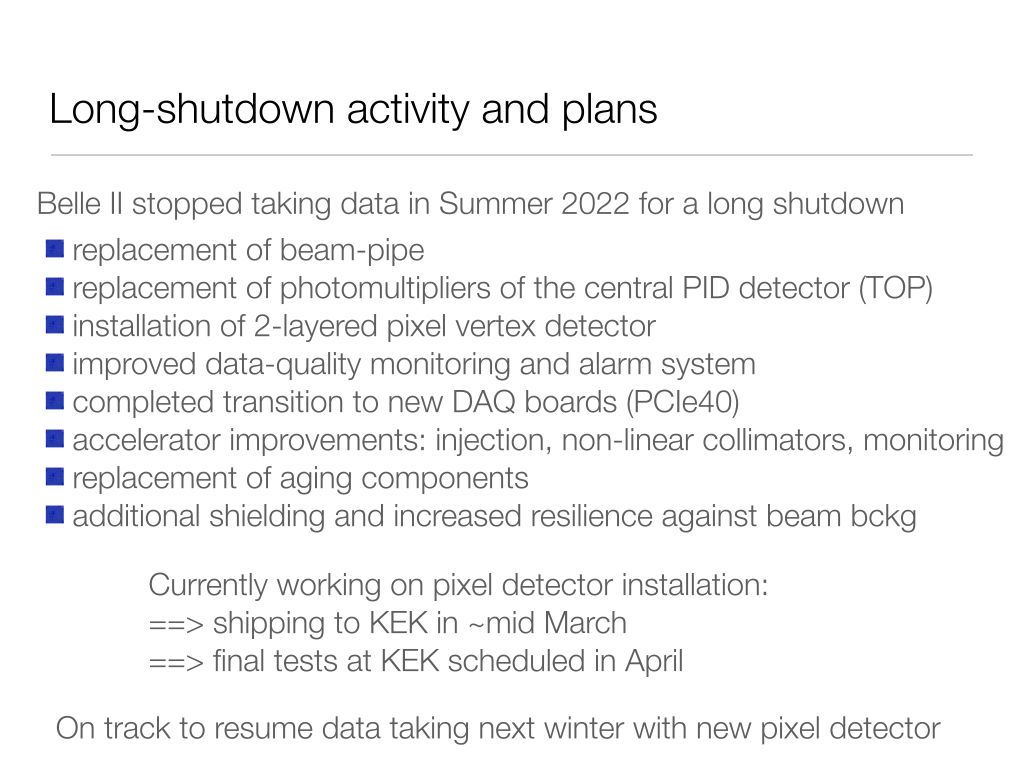
\includegraphics[page=1,width=0.95\linewidth]{slides/LS1.pdf}
\end{frame}
% %===========================================================================================================